%++++++++++++++++++++++++++++++++++++++++
% Don't modify this section unless you know what you're doing!
\documentclass[letterpaper,12pt]{article}
\usepackage{cmap} %Search in PDF
\usepackage[T2A]{fontenc} %Encoding
\usepackage[utf8]{inputenc} %Input encoding
\usepackage[english, russian]{babel}
\usepackage{tabularx} % extra features for tabular environment
\usepackage{amsmath}  % improve math presentation
\usepackage{indentfirst} %первый абзац с отстпом
\usepackage{abstract}
\usepackage{icomma}
\usepackage[dvips]{graphicx}
\graphicspath{{Pics/}}
\usepackage[margin=1in,letterpaper]{geometry} % decreases margins
\usepackage{cite} % takes care of citations\
\usepackage{wrapfig}
\usepackage[final]{hyperref} % adds hyper links inside the generated pdf file
\hypersetup{
	colorlinks=true,       % false: boxed links; true: colored links
	linkcolor=blue,        % color of internal links
	citecolor=blue,        % color of links to bibliography
	filecolor=magenta,     % color of file links
	urlcolor=blue         
}
%++++++++++++++++++++++++++++++++++++++++


\begin{document}
	
	\title{\textbf{Лабораторная работа №3}\vspace{3mm} \\ 5.1 Измерение коэффициента ослабления потока $\gamma$-лучей в веществе и определение их энергии}
	\author{Петрушенко Валерия, 5111 гр.}
	\date{Выполнено 03.10.2017}
	\maketitle
	\renewcommand{\abstractname}{\vspace{-\baselineskip}}
	
	\begin{abstract}
		С помощью сцинцтиляционного счётчика измеряются линейные коэффициенты ослабления потока $\gamma$-лучей  в свинце, железе и алюминии; по их величине определяется энергия $\gamma$-квантов.
		
	\end{abstract}
	
	
	\section{Теория}
	Гамма-лучи возникаютпри переходе возбуждённых ядер в более низкое энергетическое состояние. Энергия $\gamma$-квантов обычно порядка ~$10\div1000$ кэВ. Заряд и масса $\gamma$-кванта равны нулю. Проходячерез вещество, пучок $\gamma$-квантов ослабляется по закону:
	
	\begin{equation}
	I = I_0e^{-\mu l}
	\end{equation}
	
	
	или
	
	
	\begin{equation}
	I=I_0e^{-\mu' m_1}, 
	\end{equation}
	
	где $I, I_0$ - интенствности прошедшего и падающего излучений, $l$ - длина пути, пройденного  пучком $\gamma$-лучей	, $m_1$ - масса пройденного вещества на еденицу площади, $\mu$ и $\mu'$ - константы, зависящие от среды ($[\mu] = \text{см}^{-1}$, $[\mu'] = \text{см}^{2}/\text{г}$). $\mu'$, в отличие от $\mu$, не зависит от плотности среды. Ослабление потока    $\gamma$-лучей в веществе связано с тремя эффектами: фотоэлектрическим поглощением, комптоновским рассеянием и генерацией электрон-позитронных пар. 
	
	\vspace{0.5cm}
\textbf{Фотоэлектричекое поглощение}

	При столкновении $\gamma$-квантов с электронами внутренних атомных оболочек может происходить поглощение квантов. Свободные (наружные) электроны не могут поглощать кванты.Вероятность $dP_\text{ф}$ фотоэлектрического поглощения $\gamma$-квантов: 
	
	\begin{equation}
	dP_\text{ф}=\sigma_\text{ф} n_1 dl,
	\end{equation}

	где $dl$ - длина пути, $n_1$ - плотность внутрениних  электронов, $\sigma_\text{ф}$ - поперечное сечение отоэлектрического поглощения.
	
	\begin{equation}
	\mu_\text{ф}=\sigma_\text{ф}n_1, 
	\end{equation}
	
	$\mu_\text{ф}$ - коэффициент поглощения для фотоэффекта $\mu$ из уравнения (1).
	
	Фотоэффект является доминирующим механизмом поглощения $\gamma$-квантов при не очень высоких энергиях. Его вероятность зависит от энергии лучей и заряда  ядер.
	
	
	\begin{figure}[h]
		\centering
		{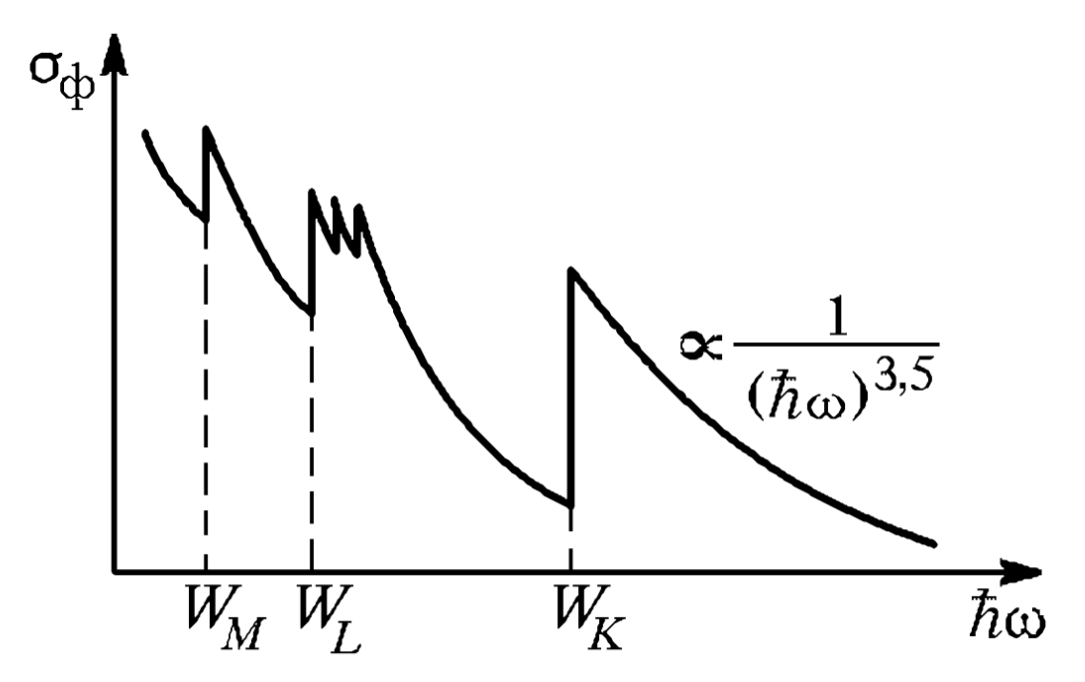
\includegraphics[width=0.45\linewidth]{01}}
		\caption{Зависимость сечения фотоэффекта от энергии $\gamma$-квантов.}
	\end{figure}
	
	
	\vspace{0.5cm}
\textbf{	Комптоновское рассеяние}


	Комптоновское рассеяние - упругое столкновение $\gamma$-кванта с электроном. Оно может происходить на свободных/слабосвязанных электронах. Эффект Комптона становится существенным, когда энергия квантов становится много больше энергии связи электронов в атоме. В этом случае сечение комптон-эффекта:
	
	\begin{equation}
	\sigma_K=\pi r^2 \dfrac{mc^2}{\hbar \omega}\left(ln\frac{2\hbar\omega}{mc^2}+\frac{1}{2}\right),
	\end{equation}
	
	где $r\simeq2,8\cdot10^{-13}$  см - классический радиус электрона, $m$ - его масса.
	
	Эффект комптона приводит не к поглощению, а к рассеянию $\gamma$-квантов и уменьшению их энергии.
	
	
	\vspace{0.5cm}
\textbf{	Образование пар}



	   При энергиях $\gamma$-лучей больше 1,02 МэВ становится возможным поглощение лучей, связанное с образованием электрон-позитронных пар. Оно возникает в электрическом поле ядер. Вероятность этого процесса приблизительно пропорциональна $Z^2$.
	   
	   \vspace{0.5cm}
	 \textbf{  Полный коэффициент ослабления потока $\gamma$-лучей}
	 
	 
	 
	Полный коэффициент ослабления потока лучей равен сумме коэффициентов для трёх рассмотренных процессов. 
	
		\begin{figure}
		\centering
		{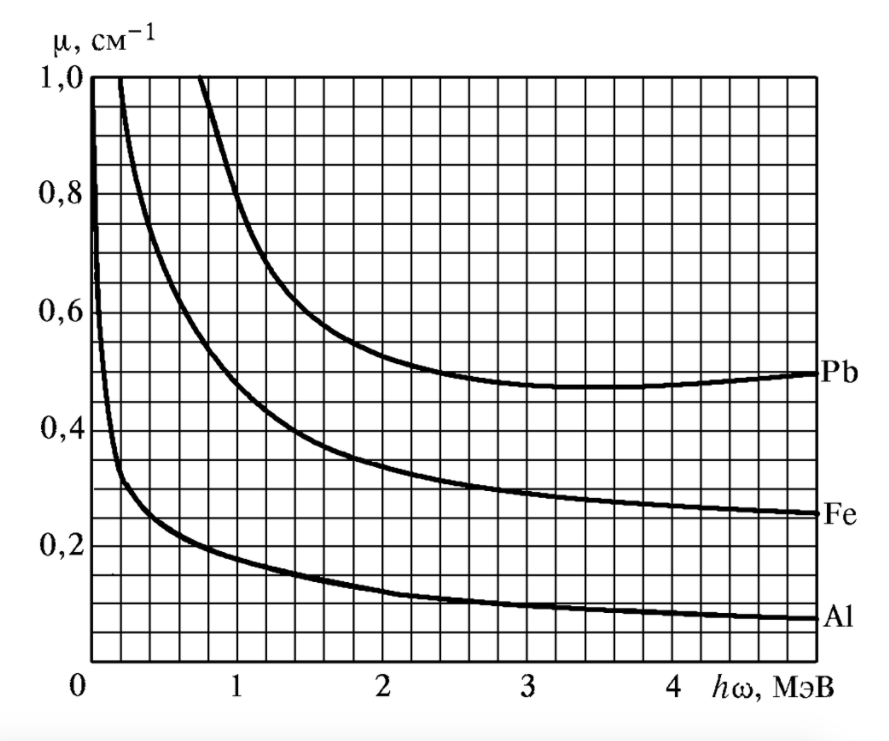
\includegraphics[width=0.5\linewidth]{02}}
		\caption{Полные коэффициенты ослабления потока $\gamma$-лучей в алюминии, железе и свинце.}
	\end{figure}
	
 	Полный коэффициент ослабления:
 	
 	\begin{equation}
 	\mu=\frac{1}{l}ln\frac{N_0}{N}
 	\end{equation}
	
	В работе определяются толщина образца $l$, число падающих частиц $N_0$  и число прошедших частиц $N$.
	
	\section{Экспериментальная установка}
	
	
		\begin{figure} [h!]
			\centering
		{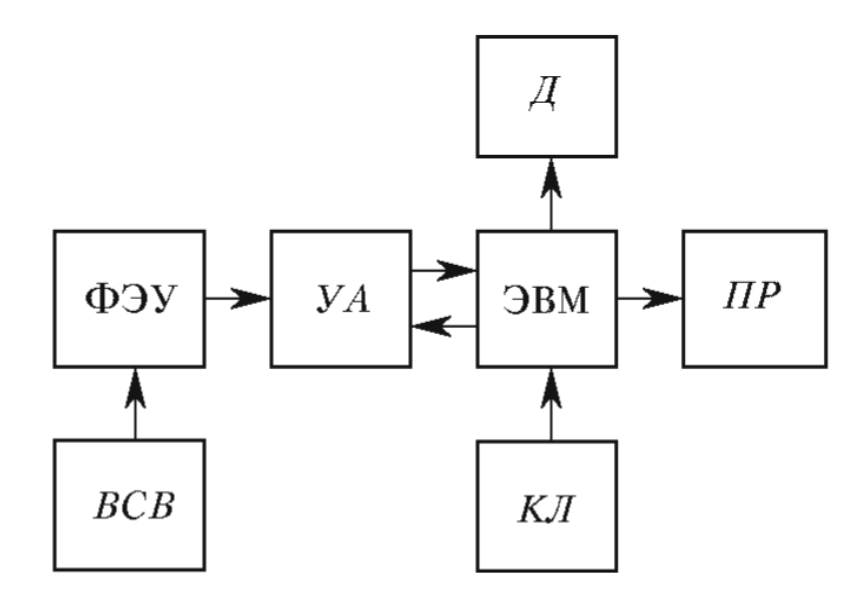
\includegraphics[width=0.8\linewidth]{03}}
			\caption{Блок-схема установки, используемой для измерения коэффициентов ослабления потока $\gamma$-лучей; Pb - свинцовый контейнер с коллиматорным каналом; П - набор поглотителей, ПП - пересчётный прибор; С - сцинтиллятор - кристалл $NaI(Tl)$; ВВ - высоковольтный выпрямитель, Ф - формирователь-выпрямитель; И - источник $\gamma$-лучей}
		\end{figure}
\pagebreak
	\begin{figure} [h!]
		\centering
		{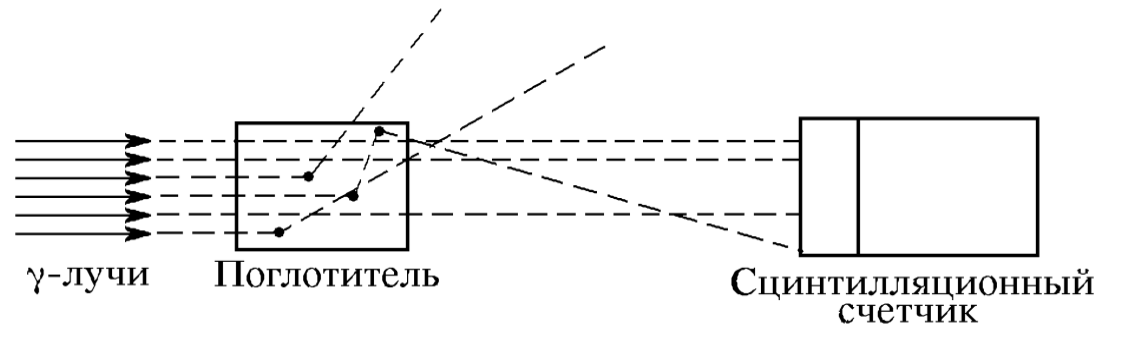
\includegraphics[width=0.9\linewidth]{04}}
		\caption{Схема рассеяния $\gamma$-квантов в поглотителе}
	\end{figure}
			
	

	\section{Ход работы}
	
	\begin{enumerate}
		\item 
	
	
	Исследовали поглощение $\gamma$-лучей в свинце, железе и алюминии. Для этого измерили число частиц, попадающих в счётчик за фиксированное время  при различной толщине образцов (точность измерения 0,3\%):  
		
			\begin{table}[h!]
				\caption{Результаты измерений для свинца:}
				\hspace{3.5cm}
				\begin{tabular}{|c||c|c|c|c|c|}
					\hline
					$l$, мм & 4 & 8 & 12 & 16 & 20 \\ \hline
					$N$, шт. & 136746 & 102354 & 105008 & 104325 & 97589  \\ \hline
					 $t_\Sigma$, с & 30 & 40 & 70 & 120 & 190 \\ \hline
				\end{tabular}
			\end{table}
		
		
			\begin{table}[h!]
				\caption{Результаты измерений для железа:}
				\hspace{3.5cm}
				\begin{tabular}{|c||c|c|c|c|c|}
					\hline
					$l$, мм & 9 & 18 & 27 & 36 & 45 \\ \hline
					$N$, шт. & 136393 & 100156 & 112720 & 103385 & 98267 \\ \hline
					$t_\Sigma$, с & 30 & 40 & 80 & 130 & 220 \\ \hline
				\end{tabular}
			\end{table}
		
		\begin{table}[h!]
			\caption{Результаты измерений для алюминия:}
			\hspace{3.5cm}
			\begin{tabular}{|c||c|c|c|c|c|}
				\hline
				$l$, мм & 20 & 40 & 60 & 80 & 100 \\ \hline
				$N$, шт. & 105329 & 102030 & 110819 & 100716 & 105235 \\ \hline
				$t_\Sigma$, с & 20 & 30 & 50 & 70 & 110 \\ \hline
			\end{tabular}
		\end{table}
		
		Абсолютная погрешность измерения толщины образца $\varepsilon_l=1$ мм.
		\item 
		
		Измерили число частиц, попадающих в счётчик за фиксированное время в отсутствие поглотителя: \underline{$N_0=166505$} частиц \underline{за 20 секунд} (точность измерения 0,3\%). Чтобы учесть фон, обусловленный шумом ФЭУ и посторонними частицами, измерили количество частиц, попадающих на счётчик за фиксированное время при закрытии коллиматора свицовой заглушкой: \underline{$N_\text{фон.}=9986$} частиц \underline{за 400 секунд} (точность измерения 0,3\%).
		Фон вычитается из всех результатов измерений.
		
		
	\end{enumerate}
		\pagebreak
		\section{Обработка данных}
				\begin{enumerate}
			\item Построили графики зависимости $ln(N-N_\text{фон.}) = f(l)$ для всех исследуемых веществ:
			
			
		\begin{figure} [h!]
		\begin{minipage}[h]{0.45\textwidth}
			\centering
			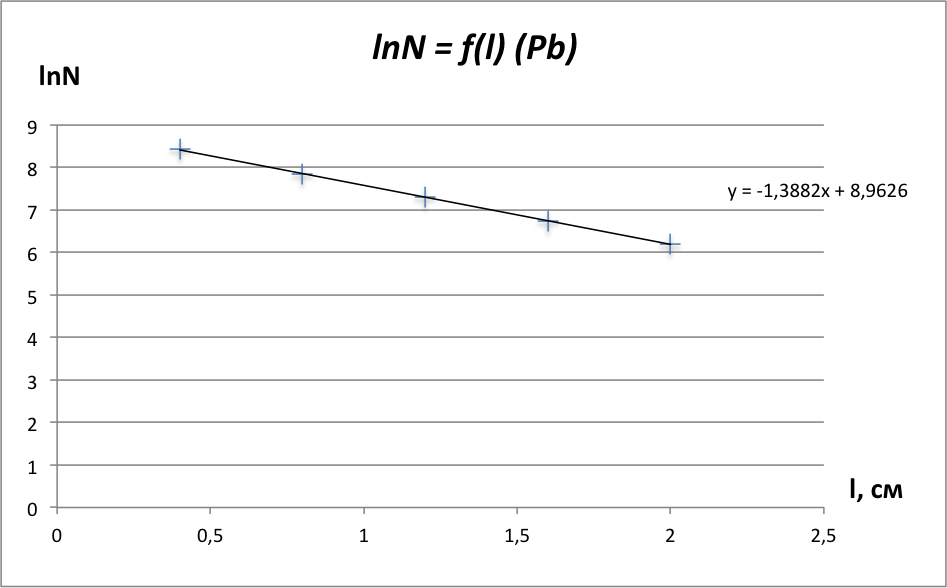
\includegraphics[width=1.2\linewidth]{05}
			\caption{График зависимости логарифма числа прошедших частиц от толщины образца для свинца}
		\end{minipage}
		\hfill
		\begin{minipage}[h]{0.45\textwidth}
			\centering
			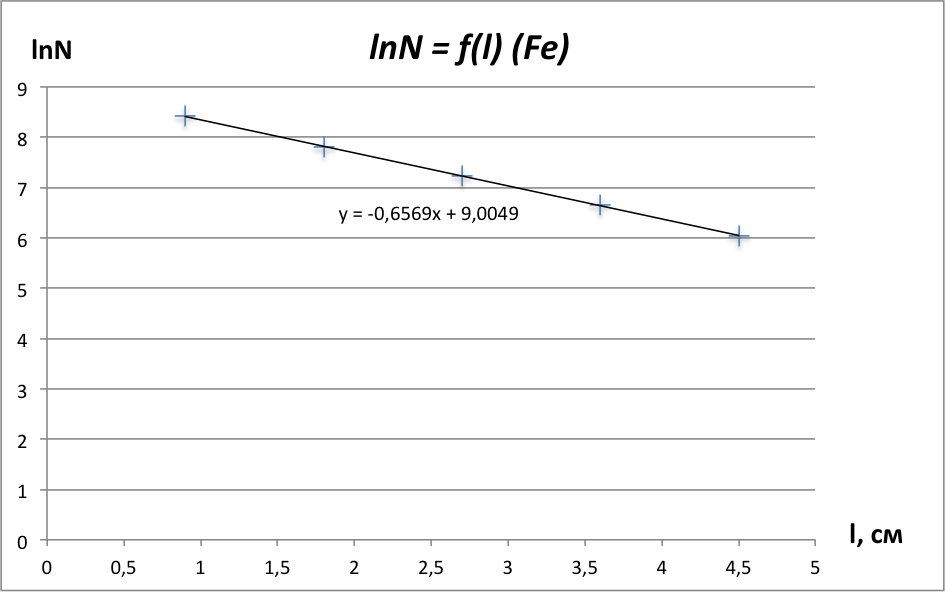
\includegraphics[width=1.2\textwidth]{06}
			\caption{График зависимости логарифма числа прошедших частиц от толщины образца для железа}
		\end{minipage}
	\end{figure}
		
		
		
		\begin{figure} [h!]
			\centering
			{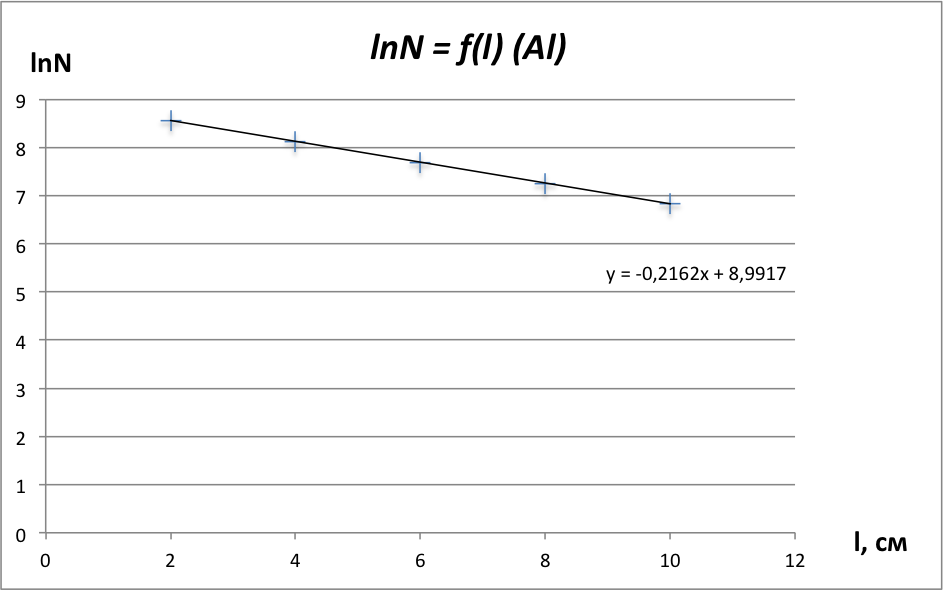
\includegraphics[width=0.6\linewidth]{07}}
			\caption{График зависимости логарифма числа прошедших частиц от толщины образца для алюминия}
		\end{figure}
		
		\item 
		С помощью графиков определили линейные коэффициенты ослабления для всех трёх веществ:
		% \vspace{-0.1cm}
		 \begin{equation}
		 \mu_{Pb}\approx1,388 ~\text{см}^{-1}
		 \end{equation}
		%\vspace{-cm}
		\begin{equation}
		\mu_{Fe}\approx0,657 ~\text{см}^{-1}
		\end{equation}
	%	\vspace{-0.7cm}
		\begin{equation}
		\mu_{Al}\approx0,216 ~\text{см}^{-1}
		\end{equation}
		
		\item 
		 По линейгым коэффициентам ослаблния нашли коэффициенты  $\mu'$  по формулам (1) и (2):
		 
		 \begin{equation}
		 \text{Из (1) и (2)} \Rightarrow \mu l = \mu' m_1
		 \end{equation}
		
		Отсюда:
		%kgjh
		\begin{equation}
		\mu'_{Pb} \approx 0,122 ~\frac{\text{см}^2}{\text{г}}
		\end{equation}
		%fgjkhf
		\begin{equation}
		\mu'_{Fe} \approx 0,084 ~\frac{\text{см}^2}{\text{г}}
		\end{equation}
		%gjf
		\begin{equation}
		\mu'_{Al} \approx 0,079 ~\frac{\text{см}^2}{\text{г}}
		\end{equation}
		
		\item 
		Используя найденные коэффициенты ослабления и табличные данные, определили среднюю энергию $\gamma$-лучей, испускаемых источником:
		
		\begin{equation}
		E_{\gamma} \sim 0,5\div0,6 ~\text{МэВ}
		\end{equation}
		
		\item 
		Рассчитали погрешности измерений:
		\begin{enumerate}
		%	\item 
	%		Погрешность измерения толщины образцов:
	%		\begin{equation*}
	%		l=1\text{мм}
	%		\end{equation*}
			\item 
			Погрешность построенных графиков, рассчитанная методом наименьших квадратов $(y=ax+b$):
			
			\begin{equation*}
			\frac{da_1}{a_1} \approx 0,005 = 0,5\%
			\end{equation*}
			
			\begin{equation*}
			\frac{da_2}{a_2} \approx 0,004 = 0,4\%
			\end{equation*}
			
			\begin{equation*}
			\frac{da_3}{a_3} \approx 0,003 = 0,3\%
			\end{equation*}
			
			
			
			
			
			
			\item 
			С учётом погрешностей:
			
			\begin{equation*}
			\mu_{Pb} = 1,388 \pm 0,007 ~\text{см}^{-1}
			\end{equation*}
			
			\begin{equation*}
			\mu_{Fe} = 0,657 \pm 0,003 ~\text{см}^{-1}
			\end{equation*}
			
			\begin{equation*}
			\mu_{Al} = 0,216 \pm 0,001 ~\text{см}^{-1}
			\end{equation*}
			
			
			
			
			
		\end{enumerate}
		
		
		\end{enumerate}
		
	
	\section{Вывод}
	Исследовали поглощение $\gamma$-лучей в свинце, алюминии и железе. Получили линейные зависимости логарифма прошедших частиц от толщины образцов и по ним определили линейные коэффициенты ослабления $\mu$ и $\mu'$, а также среднюю энергию $\gamma$-лучей, испускаемых источником.  Полученное значение составило $E_{\gamma} \sim 0,5\div0,6 ~\text{МэВ}$. Погрешности измерений не превысили 1\%.
	
	
	
\end{document}